\documentclass[titlepage, a4paper, 12pt, reqno, openany]{report}
%\documentclass[12pt]{report}
%\documentclass[titlepage, a4paper, 12pt, reqno, openany]{article}
%\documentclass[12pt]{article}
%%%%%%%%%%%%%%%%%%%%%%%%%%%%%%%%%%%%%%%%%%%%%%%%%%%%%%%%%%%%%%%%%%%%%%%%%%%%%
\usepackage{titlepic}
%%%%%%encoding%%%%%%
\usepackage[T1]{fontenc}
\usepackage[utf8]{inputenc}
\usepackage{hyphenat}
\usepackage[portuguese]{babel}
%%%%%%Hyphenation rules%%%%%%
\usepackage{graphicx} %permite inserir figuras
\usepackage[font=small,labelfont=bf]{caption} %reference figures
%\usepackage{subcaption}
\usepackage{color,colortbl,multirow}
\usepackage[top=2cm,left=1cm,right=1cm,bottom=2cm]{geometry}
%\usepackage[margin=2cm]{geometry} %margens
%\usepackage[left=2cm,top=1cm,bottom=2cm,right=3cm,nohead,nofoot]{geometry}
\usepackage{paralist}
\usepackage{float}
\usepackage{verbatim}
\usepackage{lipsum}
\usepackage{multicol}
\usepackage{babelbib}
\usepackage{amsfonts}
\usepackage{amsmath}
\usepackage{amssymb}
%%%%%%%%%%%%%%%%%%%%%%%%%%%%%%%%%%%%%%%%%%%%%%%%%%%%%%%%%%%%%%%%%%%%%%%%%%%%%%%
\usepackage[usenames,dvipsnames,svgnames,table]{xcolor} %\usepackage[usenames]{color} %permite letras coloridas
\usepackage{adjustbox}
\usepackage{makecell}
%\usepackage{times}
%\usepackage{makeidx} %para criar índice remissivo
%\usepackage{array}
%\usepackage{supertabular}
%\usepackage{bm}
%\usepackage{booktabs}
%\usepackage{boxedminipage}
%\usepackage{caption}
%\usepackage{changepage}
%\usepackage{cite}
%\usepackage{easylist}
%\usepackage{esint}
%\usepackage{eucal}
%\usepackage{fancyhdr}
%\usepackage{hyperref} %index dentro de red boxes
%\usepackage{indentfirst}
%\usepackage{latexsym}
%\usepackage{listings}
%\usepackage{mathptmx}
%\usepackage{mathrsfs} %permite o uso de letras trabalhadas
%\usepackage{microtype}
%\usepackage[normalem]{ulem} %permite sublinhar palavras
%\usepackage{pifont}
%\usepackage{rotating}
%\usepackage{setspace}
%\usepackage{syntonly} %speedup work desabling pdf converse \syntaxonly
%\usepackage{subfiles}
%\usepackage{textcomp}
%\usepackage{theorem}
%\usepackage{ulem}
%\usepackage{url}
%\usepackage{wrapfig}
%%%%%recent%%%%%
%\usepackage{cancel}
%\usepackage[fleqn]{mathtools}
%\usepackage{pdfpages}
%\usepackage{pdflscape}
%\usepackage{todonotes}
%\usepackage{siunitx}
%%%%%%%%%%%%%%%%%%%%%%%%%%%%%%%%%%%%%%%%%%%%%%%%%%%%%%%%%%%%%%%%%%%%%%%%%%%%%%%%%%%
%\renewcommand\thesection{\arabic{section}}
%\renewcommand\thesubsection{\thesection.\arabic{subsection}}
%%%%%%%%%%%%%%%%%%%%%%%%%%%%%%%%%%%%%%%%%%%%%%%%%%%%%%%%%%%%%%%%%%%%%%%%%%%%%%%%%%%%
\begin{comment}
\usepackage{enumitem}
\setlistdepth{12}
\newlist{enumitem}{enumerate}{12}
\setlist[enumitem,1]{label=\roman*)}
\setlist[enumitem,2]{label=\alph*)}
\setlist[enumitem,3]{label=\arabic*)}
\setlist[enumitem,4]{label=(\roman*)}
\setlist[enumitem,5]{label=(\alph*)}
\setlist[enumitem,6]{label=(\arabic*)}
\setlist[enumitem,7]{label=\roman*)}
\setlist[enumitem,8]{label=\alph*)}
\setlist[enumitem,9]{label=\arabic*)}
\setlist[enumitem,10]{label=(\roman*)}
\setlist[enumitem,11]{label=(\alph*)}
\setlist[enumitem,12]{label=(\arabic*)}
\end{comment}

%%%%%%%%%%%%%%%%%%%%%%%%%%%%%%%%%%%%%%%%%%%%%%%%%%%%%%%%%%%%%%%%%%%%%%%%%%%%%%%%%%%%
\begin{comment}
\usepackage{enumerate}
\renewcommand{\labelitemi}{$\bullet$}
\renewcommand{\labelitemii}{$\cdot$}
\renewcommand{\labelitemiii}{$\diamond$}
\renewcommand{\labelitemiv}{$\ast$}
\end{comment}

%%%%%%%%%%%%%%%%%%%%%%%%%%%%%%%%%%%%%%%%%%%%%%%%%%%%%%%%%%%%%%%%%%%%%%%%%%%%%%%%%%%%
\begin{comment}
\usepackage{tikz}
\usepackage{circuitikz}
\usetikzlibrary{matrix,shapes.geometric,arrows,trees,positioning,calc}
%%%%%%%%%%%%%%%%%%%%%%%pre defined figures%%%%%%%%%%%%%%%%%%%%%
\tikzstyle{RECTANGLE_2} = [rectangle, draw, text width=5em, text centered, rounded corners, minimum height=4em]
\tikzstyle{RECTANGLE_3} = [rectangle, rounded corners, minimum width=3cm, minimum height=1cm,text centered, draw=black, fill=red!80]
\tikzstyle{RECTANGLE_4} = [rectangle, draw, fill=blue!20, text width=3cm, text centered, minimum height=4em]
\tikzstyle{RECTANGLE_5} = [rectangle, minimum width=3cm, minimum height=1cm, text centered, text width=3cm]
\tikzstyle{RECTANGLE_6} = [rectangle, draw, fill=blue!20, text width=5em, text centered, rounded corners, minimum height=4em]
\tikzstyle{RECTANGLE_7} = [rectangle, draw, fill=blue!20, text width=5em, text centered, rounded corners, minimum height=4em]
\tikzstyle{RECTANGLE_8} = [rectangle, draw, align=left, fill=blue!20]
\tikzstyle{RECTANGLE_1} = [rectangle, rounded corners, minimum width=1cm, minimum height=1cm,text centered, draw=black, fill=green!%30]
\tikzstyle{DIAMOND_1} = [diamond, draw, fill=blue!20, text width=4.5em, text badly centered, node distance=4cm, inner sep=0pt]
\tikzstyle{DIAMOND_2} = [diamond, minimum width=3cm, minimum height=1cm, text centered, draw=black, fill=green!30]
\tikzstyle{DIAMOND_3} = [diamond, draw, text width=4.5em, text badly centered, node distance=3cm, inner sep=0pt]
\tikzstyle{DIAMOND_4} = [diamond, draw, fill=blue!20, text width=4.5em, text badly centered, node distance=3cm, inner sep=0pt]
\tikzstyle{DIAMOND_5} = [diamond, draw, fill=blue!20, text width=4.5em, text badly centered, node distance=3cm, inner sep=0pt]
\tikzstyle{DIAMOND_6} = [diamond, draw, fill=blue!20, text width=4.5em, text badly centered, node distance=4cm, inner sep=0pt]
\tikzstyle{DIAMOND_7} = [diamond, draw, align=left, fill=blue!20]
\tikzstyle{ELLIPSE_1} = [draw, ellipse,fill=red!20, node distance=3cm, minimum height=2em]
\tikzstyle{ELLIPSE_2} = [draw, ellipse,fill=red!20, node distance=3cm, minimum height=2em]
\tikzstyle{ELLIPSE} = [draw, ellipse,fill=red!20, node distance=3cm, minimum height=2em]
\tikzstyle{TRAPEZIUM_1} = [trapezium,trapezium left angle=70,trapezium right angle=-70,minimum height=0.6cm, draw, fill=blue!20, text width=4.5em, text badly centered, node distance=3cm, inner sep=0pt]
\tikzstyle{TRAPEZIUM_2} = [trapezium, trapezium left angle=70, trapezium right angle=110, minimum width=3cm, minimum height=1cm, text centered, draw=black, fill=blue!30]
\tikzstyle{TRAPEZIUM_3} = [trapezium,trapezium left angle=70,trapezium right angle=-70,minimum height=0.6cm, draw, fill=blue!20, text width=4.5em, text badly centered, node distance=3cm, inner sep=0pt]
\tikzstyle{ARROW} = [thick,->,>=stealth]
\tikzstyle{LINE} = [draw, -latex']
\tikzstyle{MYLINE} = [draw, ->,  thick, shorten <=4pt, shorten >=4pt]
\tikzstyle{TEXT_1}=[draw,text centered,minimum size=6em,text width=5.25cm,text height=0.34cm]
\tikzstyle{TEXT_2}=[draw,text centered,minimum size=2em,text width=2.75cm,text height=0.34cm]
\tikzstyle{TEXT_3}=[draw,minimum size=2.5em,text centered,text width=3.5cm]
\tikzstyle{TEXT_4}=[draw,minimum size=3em,text centered,text width=6.cm]
\tikzstyle{CIRCLE_1}=[draw,shape=circle,inner sep=2pt,text centered, node distance=3.5cm]
\tikzstyle{CIRCLE_2}=[draw,shape=circle,inner sep=4pt,text centered, node distance=3.cm]
\end{comment}

%%%%%%%%%%%%%%%%%%%%%%%%%%%%%%%%%Not Adviced%%%%%%%%%%%%%%%%%%%%%%%%%%%%%%%%%%%%%%%%
%\usepackage{showidx} %for troubleshooting index
%\usepackage{showkeys} %for troubleshooting \label \ref
%\usepackage{pxfonts}

%%%%%%%%%%%%%%%%%%%%%%%%%%%%%%%%%claching Package%%%%%%%%%%%%%%%%%%%%%%%%%%%%%%%%%%%
%\usepackage{pgfplots}
%\usepackage{natbib}
%\usepackage[usenames]{color} %permite letras coloridas
%\usepackage{xypic}

%%%%%%%%%%%%%%%%%%%%%%%%%%%%%%%%%Not Installed Yet%%%%%%%%%%%%%%%%%%%%%%%%%%%%%%%%%%

%%%%%%%%%%%%%%%%%%%%%%%%%%%%%%%Com Dependencias%%%%%%%%%%%%%%%%%%%%%%%%%%%%%%%%%%%%%
%\usepackage{glossaries}
%\usepackage[version=3]{mhchem}

%%%%%%%%%%%%%%%%%%%%%%%%%%%%%%%%%%%%%%%%%%%%%%%%%%%%%%%%%%%%%%%%%%%%%%%%%%%%%%%%%%%%
% alguns pacotes nao sao reconhecidos, ter atencao quais usar em differents computadores, tambem alguns pacotes entram em conflito.
\newtheorem{theorem}{Theorem}
\newtheorem{lemma}{Lemma}
\newtheorem{definition}{Defini\c{c}\~{a}o}
\newtheorem{notation}{Notation}

%%%%%%%%%%%%%%%%%%%%%%%%%%%%%%%%Not Working%%%%%%%%%%%%%%%%%%%%%%%%%%%%%%%%%%%%%%%%%
%\usepackage{itemize}
%\usepackage{named}
%\usepackage{amscls}
%\usepackage{fullpage}

%%%%%%%%%%%%%%%%%%%%%%%%%%%%%%%%%%%%%%%%%%%%%%%%%%%%%%%%%%%%%%%%%%%%%%%%%%%%%%%%%%%%
%\usepackage{apacite} %Bibliography style
%%%%%%%%%%%%%%%%%%%%%%%%%%%%%%%%%%%%%%%%%%%%%%%%%%%%%%%%%%%%%%%%%%%%%%%%%%%%%%%%%%%%
\makeindex
%%%%%%%%%%%%%%%%%%%%%%%%%%%%%%%%%%%%%%%%%%%%%%%%%%%%%%%%%%%%%%%%%%%%%%%%%%%%%%%%%%%%
\begin{document}
%\bibliographystyle{apacite}
\bibliographystyle{babplain}
%%%%%%%%%%%%%%%%%%%%%%%%FIX SECTION NUMBERING IN CASE REPORT%%%%%%%%%%%%%%%%%%%%%%%%
\renewcommand\thesection{\arabic{section}}
\renewcommand\thesubsection{\thesection.\arabic{subsection}}
\renewcommand\thesubsubsection{\thesection.\thesubsection.\arabic{subsubsection}}

\begin{minipage}{\linewidth}

\title{Comportamento Organizacional}
\author{
\emph{S\'{e}rgio Santos},\;$N^o$:\; 1020881 \\
\emph{Nome 2},\;$N^o$:\; 2000000\\
\emph{Nome 3},\;$N^o$:\; 3000000\\
%\emph{Nome 4},\;$N^o$:\; 4000000\\
%\emph{Nome 5},\;$N^o$:\; 5000000\\
}
\date{\today}
%\titlepic{
\includegraphics[scale=0.50]{./image/ROQ/ROQ.jpg}}

\begin{titlepage}

\includegraphics[scale=0.60]{./image/capa/ISEP_marca_cor_grande.png}
\maketitle
\vspace{8cm}
\begin{flushleft}

\includegraphics[scale=0.50]{./image/ROQ/ROQ.jpg}
\end{flushleft}
\end{titlepage}

\end{minipage}

\tableofcontents
\appendix
\pagestyle{plain} %plain headings empty
%\setcounter{chapter}{0}
%\numberwithin{page}{section}
%\renewcommand{\abstractname}{Executive Summary}
\setlength{\parindent}{0in}
%%%%%%%%%%%%%%%%%%%%%%%%%%%%%%%%%%%%%%%%%%%%%%%%%%%%%%%%%%%%%%%%%%%%%%%%%%%%%%%%%%%%%%%%%%%%%%%%%%%%%%%%%%%%%%%
\label{Resumo}
\begin{abstract}
Abstract
\end{abstract}
%%%%%%%%%%%%%%%%%%%%%%%%%%%%%%%%%%%%%%%%%%%%%%%%%%%%%%%%%%%%%%%%%%%%%%%%%%%%%%%%%%%%%%%%%%%%%%%%%%%%%%%%%%%%%%%
\newpage
\section{Introdução}
%%%%%%%%%%%%%%%%%%%%%%%%%%%%%%%%%%%%%%%%%%%%%%%%%%%%%%%%%%%%%%%%%%%%%%%%%%%%%%%
\qquad A juventude foi ensinada que a missão de se tornarem adultos, o caminho de dignidade, segurança e independência é obter um emprego.\\
O estagio sendo importante para qualquer iniciante de qualquer profissão de forma a ser transmitido conhecimentos adquiridos, que em certas profissões pode demorar até alguns anos para alcançar a categoria de oficial ou sénior.\\

more stuff, and more.


\begin{minipage}[t]{\linewidth}
\quad Opcões:
\begin{itemize}
\setlength\itemsep{-0.3em}
\item Trabalhador por conta de outrem
\begin{itemize}
\item Organização privada
\item Organização publica
\begin{figure}[H]
\centering
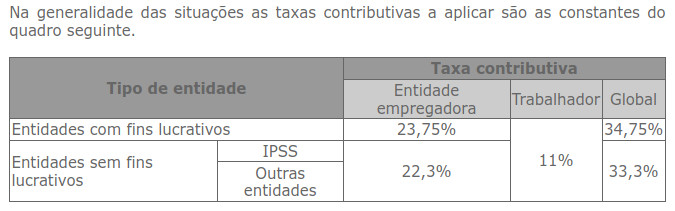
\includegraphics[scale=0.52]{./image/SGS/Contribuicoes_1.jpg}
\caption{Contribuições para SGS}
\end{figure}\par
Como podemos ver o cidadão nesta situação desconta, 34,5\% e 33,3\% respetivamente para o estado.\\
Exemplo: se um vencimento é de 1000Eur será descontado 11\% para a Segurança Social, ficando com $1000\times (1-0,11)=890Eur$ e a empresa desconta por ti por exemplo 34,5\%, que dá $1000\times 0,345=345EUR$, ao todo será descontado $110+345=455Eur$, ou seja, todos os messes um trabalhador que ganhe 1000EUR desconta para a Segurança Social direto e indiretamente \textbf{455Eur}.\\
Na realidade o vencimento neste exemplo do cidadão é de \textbf{1345Eur}, o seja, é prejudicado nos seus descontos na quantia de 345Eur [34,5\%] pois não são considerados mais tarde para a reforma.\\
A circulação deste capital passa despercebido e usado pelo estado para seus gastos, sendo o cidadão sua fonte, sem nenhum proveito, a não ser as empresas que depois recebem ajudas através desta receita.\\
Em Geral a receita laboral de um cidadão é quase metade $34,5\%+11\%=45,5\%$ depois dos respetivos descontos [1000Eur \textit{vs} 455Eur].\\
Estas contas são feitas sem considerar qualquer subsidio de alimentação.
\end{itemize}
\item Trabalhadores independentes
\begin{itemize}
\item Recibos Verdes
\item Recibos Verdes Falsos\\ \\
Este tipo de trabalhador em principio pode definir seus descontos numa dada margem, e aliciante para as empresas pois não tem qualquer responsabilidade futura, acarretando toda a responsabilidade para o trabalhador independente na qual em principio ira ganhar mais doque o por outrem, mas descontando muito menos e prejudicado a longo prazo devido a concorrência, a não ser que desconte a totalidade de $34,5\%+11\%=45,5\%$ e ainda obter um vencimento superior ao equivalente do trabalhador por outrem.
\end{itemize}
\item Trabalhador do serviço domestico
\item Membros de órgãos estatuários
\item Empresario
\begin{itemize}
\item Serviços
\item Bens\\ \\
\end{itemize}
\end{itemize}
\end{minipage}\par
Nenhum cidadão deve aceitar qualquer trabalho que ganhe menos que $ \mbox{\Large $ \frac{635Eur}{0,65} $ } $, pois 635Eur é o salario mínimo nacional, e se ficar em \textit{lay off} ou \textit{desempregado}, como demonstrado:\\
$635\times(1-0,11)\approx566Eur$,\\
$635\times(0,345)\approx220Eur$,\\
pois estará a trabalhar gratuitamente, só ira receber \textbf{566Eur} e desconta \textbf{289Eur}, ou seja um escravo do estado.\\
















\subsection{O futuro do trabalho}
\qquad Agora com as novas tecnologias tem se aberto várias portas para novas formas de as pessoas serem remuneradas por seus serviços ou bens. Exemplos muito notórios são casos como a UBER, AMAZON, YOUTUBE, LINKEDIN, etc.\\

Esta a fugir para uma forma de trabalhadores independentes, controlado por sistemas tecnológicos administrativos, empresas virtuais, que pode ser formas de exploração e concorrência desleal, quando mal usados, que proporcionam enriquecimento rápido aos que implementem estes sistemas e o gerem.



\subsection{A gestão de carreira e as competências necessárias num mundo em mudança}

shows that workers in digital-intensive industries on average exhibit higher levels of cognitive as well as non-cognitive skills and social skills than workers in less digitally-intensive sectors of the economy. This may of course depend on the type of workers employed in digital vs less digital intensive sectors, with the latter being generally more intensive in unskilled workers.\\

Skills are better rewarded in digital intensive sectors\\

Table 2 shows that for two types of skills, labour market returns are higher in digital intensive industries than in less digital intensive industries. These are advanced numeracy skills and self-organisation skills.\\

these results are robust to a number of checks. In Table A2, each interaction term enters the specification alone (rather than introducing all interaction terms at the same time, as in Table 2). The results show that all type of skills are better rewarded in digital intensive industries, in particular advanced numeracy skills, self-organisation skills, ICT skills and numeracy. However, in these specifications the estimated coefficients for the skill variables are clearly biased upwards by the omission of all other skill variables, which are correlated with the individually included skill.\\

geração Z em 2025 faz parte de 75% da classe trabalhadora.

Wage returns to ICT skills are twice as big as those related to numeracy skills, whereas management and communication skills are rewarded as much as numeracy skills are. These results also indicate the importance for workers to adequately use their skills and human capital on the job. This in turns calls for workers to be well matched to tasks they perform on the job and stresses the importance of good human resource and organisational management within firms.

the returns to task-based skills are still in the same ballpark than those for cognitive skills constitutes strong evidence about the importance of task-specific human capital for production and labour markets. Wage returns to ICT skills are twice as big as those related to numeracy skills, whereas management and communication skills are rewarded as much as numeracy skills are. These results also indicate the importance for workers to adequately use their skills and human capital on the job. This in turns calls for workers to be well matched to tasks they perform on the job and stresses the importance of good human resource and organisational management within firms.\\

Workers in digital intensive sectors are generally better paid\\

Only Deming (2015), who uses data on cognitive and non-cognitive skills for workers in the U.S., finds that in ICT intensive jobs bundles of cognitive and non-cognitive skills are better rewarded.\\

Especially in digital intensive industries, the production process might be more decentralised (as e.g. outsourcing, offshoring and vertical integration may occur more frequently) and the bundling of self-organisation and management and communication with advanced numeracy skills is key to ensure the functioning of production and the workflow within teams.\\

The findings indicate that cognitive as well as non-cognitive skills are strongly rewarded by labour markets, even when controlling for industry and occupation fixed effects, individual control variables (including education) and firm size. In addition, the fact that the returns to task-based skills are still in the same ballpark than those for cognitive skills highlights the importance of task- specific human capital for production and labour markets. Wage returns to ICT skills are twice as large as those to numeracy skills, whereas management and communication skills are almost equally rewarded as numeracy skills.\\

Furthermore, the results show that digital intensive industries reward workers having relatively higher levels of self-organisation and advanced numeracy skills more than less digital intensive industries. Moreover, for workers in digital intensive industries, bundles of skills are particularly important: workers endowed with a high level of numeracy skills receive an additional wage premium, if they also show high levels of self-organisation or managing and communication skills. Thus, the present analysis contributes to inform policy makers on the relationship between the digital transformation and skills’ needs and supply. This is essential for the design of effective and forward-looking skills and employment policies, aimed at aligning labour market demand and supply and at fostering productivity.\\

Understanding which skills, cognitive as well as non-cognitive, yield high returns in the labour market is also important to address inequality issues and to foster employment and well-being. If the demand of certain skills and certain bundles of skills outgrow the supply for such skills, the rewards of these skills would increase while those for other skills would decline. This skill shortage could easily lead to rising wage inequality and even to a surge of unemployment of workers not possessing these types of skills. For this reason, to curb the rising wage inequality, it may be important to design or target training programs so that they better prepare workers for the specific skills being high in demand, given the acceleration of the digital transformation across occupations and industries. Moreover, the earlier the training takes place, the lower the costs of trainings for cognitive as well as non-cognitive skills become (Cunha and Heckman, 2007; Cunha et al., 2010). Therefore, recognising major skills needed for digitalisation is important not only for labour market policy interventions, but also for policies specifically targeting the education sector.\\

Finally, as the digital transformation will soon also affect industries that are at present less digitalised, governments will more and more need to equip their populations with a wide range of skills, and to continue doing so over time. This might entail not only strengthening quantitative or cognitive skills, but also combining these with a good endowment of non-cognitive and socio-emotional skills. The proposed work can therefore help countries identifying the sets of key skills their citizens need to be equipped with to succeed in the digital era. This is important for the design and implementation of education and training programmes, as well as to enhance labour market participation and workers’ performance.\\

The research on personality traits (or non-cognitive skills), especially for North America, has been organised following the so-called "Big Five" factor model of personality (Goldberg, 1990). This suggests that most personality measures could be subsumed under an umbrella including five key factors:
extraversion, agreeableness, conscientiousness (or dependability), emotional stability (vs. neuroticism), and openness to experience.\\


EU and national governments aim vocational education and training. But how do
to close the skills gap and increase digital European workers see the need for action in order skills signifi cantly through a wide range of to equip themselves with all the skills necessary for initiatives, one of the most important being Industry 4.0?




\subsection{plano de desenvolvimento pessoal de competências}

que o aluno considere
fundamentais no contexto do trabalho do futuro, para atingir os seus objetivos
profissionais. Para tal, deverá:
a) Realizar um diagnóstico de competências pessoais;
b) Definir objetivos de carreira;
c) Definir as competências que considere que no futuro lhe permitirão atingir os
referidos objetivos;
d) Definir um plano de desenvolvimento para as competências anteriormente
selecionadas.
• A componente individual do trabalho a realizar por cada aluno deverá ser entregue em forma de um padlet (https://padlet.com) que demonstre todas as pesquisas e inputs a que o aluno recorreu para a realização do trabalho bem como as suas reflexões. O padlet deve terminar com a apresentação do plano de
desenvolvimento pessoal de competências.
• Cada aluno deverá defender oralmente a componente individual.


\newpage
\section{Conclusão}
%%%%%%%%%%%%%%%%%%%%%%%%%%%%%%%%%%%%%%%%%%%%%%%%%%%%%%%%%%%%%%%%%%%%%%%%%%%%%%%%%%%%%%%%%%%%%%%%%%%%%%%%%%%%%%%%%%%%%%%%%%%%%%%%%%%%%%%%%%%%%%%%%%%%%%%%%%%%%%
\newpage
%%%%%%%%%%%%%%%%%%%%%%%%%%
%\part*{Equa\c{c}\~{o}es} \label{eq}
%
\begin{flushleft}
{\bf Corrente Continua Condi\c{c}\~{o}es \index{Condi\c{c}\~{o}es} iniciais \index{iniciais} nulas \index{nulas}.}\par
\end{flushleft}
 \quad Circuito \index{Circuito} $LC$ em $C.C$:\par
%
\begin{itemize}
\item
$i(t)=\frac{V_{DC}\sqrt{LC}}{L}\quad \sin \left( \frac{t}{\sqrt{LC}}\right)\times u(t)$\par
\item
$V_L(t)=V_{DC}\quad \cos\left(\frac{t}{\sqrt{LC}} \right)\times u(t)$\par
\item
$V_c(t)=V_{DC}\quad \left(1-\cos\left(\frac{t}{\sqrt{LC}} \right) \right)\times u(t)$\par
\item
$\omega_n=\frac{1}{\sqrt{LC}}$\par
\item
$\overline{Z}=\sqrt{(\omega_n L-\frac{1}{\omega_n C})^2}$\par
\item
$\phi_p=\frac{\pi}{2}$\par
porque, $\sin(\omega_n t)= \cos(\omega_n t - \pi/2)$\par
\item
$\tau=\infty$\par
\end{itemize}
%
%%%%%%%%%%%%%%%%%%%%%
\quad Circuito \index{Circuito} $RLC$ em $C.C$:\par
%
\begin{enumerate}
%enum1
\item
Para \quad $C(C R^2-4 L)>0$ \quad (Ra\'{i}zes \index{Ra\'{i}zes} reais \index{reais} diferentes \index{diferentes}) \quad Sobreamortecido \index{Sobreamortecido}.\par
%
\begin{itemize}
\item
$i(t)=\frac{2 V_{DC} C e^{\frac{-tR}{2L}} sinh \left( \frac{t \sqrt{C(CR^2-4L)}}{2CL} \right)}{\sqrt{C(CR^2-RL)}}\times u(t)$\par
\item
$V_R(t)=R\times i(t)$\par
\item
$V_L(t)=L\dfrac{di(t)}{dt}$\par
%
\begin{minipage}{0.95\linewidth}
\makebox[\linewidth]{
\includegraphics[scale=0.75]{./Image/equacoes_1.png}
}
\end{minipage}\par
%
\item
$V_C(t)=\frac{1}{C}\int_0^ti(t)$\par
%
\begin{minipage}{0.95\linewidth}
\makebox[\linewidth]{
\includegraphics[scale=0.75]{./Image/equacoes_2.png}
}
\end{minipage}\par
%
\end{itemize}
%enum2
\item
Para \quad $C(C R^2-4 L)=0$ \quad (Ra\'{i}zes \index{Ra\'{i}zes} iguais \index{iguais})\quad Amortecimento \index{Amortecimento} cr\'{i}tico \index{cr\'{i}tico}.\par
%
\begin{itemize}
\item
$i(t)=\frac{V_{DC}}{L} \quad  t \quad e^{\frac{-R t}{2L}} \times u(t)$\par
\item
$V_R(t)=R\times i(t)$\par
\item
$V_L(t)=L\dfrac{di(t)}{dt}$\par
%
\begin{minipage}{0.95\linewidth}
\makebox[\linewidth]{
\includegraphics[scale=0.75]{./Image/equacoes_3.png}
}
\end{minipage}\par
%
\item
$V_C(t)=\frac{1}{C}\int_0^ti(t)$\par
\begin{minipage}{0.95\linewidth}
\makebox[\linewidth]{
\includegraphics[scale=0.75]{./Image/equacoes_4.png}
}
\end{minipage}\par
%
\end{itemize}
%enum3
\item
Para \quad $C(C R^2-4 L)<0$ \quad (Ra\'{i}zes \index{Ra\'{i}zes} complexas \index{complexas}) \quad Amortecido \index{Amortecido}.\par
%
\begin{itemize}
\item
$i(t)=\frac{2 V_{DC} C e^{\frac{-tR}{2L}} sin \left( \frac{t \sqrt{-C(CR^2-4L)}}{2CL} \right)}{\sqrt{-C(CR^2-4L)}}\times u(t)$\par
\item
$V_R(t)=R\times i(t)$\par
\item
$V_L(t)=L\dfrac{di(t)}{dt}$\par
%
\begin{minipage}{0.95\linewidth}
\makebox[\linewidth]{
\includegraphics[scale=0.75]{./Image/equacoes_5.png}
}
\end{minipage}\par
%
\item
$V_C(t)=\frac{1}{C}\int_0^ti(t)$\par
%
\begin{minipage}{0.95\linewidth}
\makebox[\linewidth]{
\includegraphics[scale=0.75]{./Image/equacoes_6.png}
}
\end{minipage}\par
%
\end{itemize}
\end{enumerate}
%
\begin{itemize}
\item
$| \omega_n |=\sqrt{\frac{4 L-R^2 C}{4 L^2 C}}$\par
\item
%\overrightarrow{Z}
$\overline{Z}=\sqrt{R^2 + (\omega_n L -\frac{1}{\omega_n C})^2}$\par
\item
$\phi_p=\arctan\left(\frac{\omega_n L - \frac{1}{\omega_n C}}{R}\right)$\par
\item
$\tau=\frac{2 L}{R}$\par
\end{itemize}
%%%%%%%%%%%%%%%%%%%%%%%%%%%%%%%%%%%%%%%%%%
\begin{flushleft}
{\bf Corrente \index{Corrente} Alternada condi\c{c}\~{o}es \index{Condi\c{c}\~{o}es} iniciais \index{iniciais} nulas \index{nulas}}.
\end{flushleft}
\quad Circuito \index{Circuito} $RLE$ em $C.A$:\par
\begin{itemize}
\item
$i(t)=C_T\ e^{-\frac{R}{L}t}+\frac{V_{m\acute{a}x}}{\overline{Z}}\sin(\omega t + \alpha - \phi_p)-\frac{E}{R}$\newline
$i(t)=C_T\ e^{-\frac{R}{L}t} + C_1 \cos (\omega t) + C_2 \sin(\omega t)-\frac{E}{R}$
\item
$I(\omega t)=C_T\ e^{-\frac{R}{L \omega}\omega t}+\frac{V_{m\acute{a}x}}{\overline{Z}}\sin(\omega t + \alpha - \phi_p)-\frac{E}{R}$
\item
$\overrightarrow{Z}=R+j\omega L$\\
$\overline{Z}=\sqrt{R^2 + (\omega L)^2}$
\item
$\phi_p=\arctan(\frac{\omega L}{R})$
\item
$C_T=\frac{E}{R}-\frac{V_{m\acute{a}x}}{\overline{Z}}\sin(\alpha - \phi_p)$
\item
$C_T=\frac{V_{m\acute{a}x}}{R^2 + (\omega L)^2}(L \omega \cos(\alpha) - R \sin (\alpha))+\frac{E}{R}$
\item
$C_1=\frac{V_{m\acute{a}x}}{R^2 + (\omega L)^2}(R \sin (\alpha) - L \omega \cos(\alpha))$
\item
$C_2=\frac{V_{m\acute{a}x}}{R^2 + (\omega L)^2}(R \cos (\alpha) + L \omega \sin (\alpha))$
%
\end{itemize}
%%%%%%%%%%%%%%%%%%%%%%%
%\part*{Defini\c{c}\~{o}es} \label{def}
\begin{definition}
Capacit\^{a}ncia
\begin{flalign*}
Q_c(t) =& \int^t i(t) \quad dt & \\
=& Q_c(0^-)+\int_{0^-}^t i(t) \quad dt & \\
V_c(t) =& \frac{Q_c(t)}{C} & \\
=& \frac{1}{C} \quad \int^t i_c(t) \quad dt & \\
=& \frac{Q_c(0^-)}{C} + \frac{1}{c} \quad \int_0^t i_c(t) \quad dt & \\
=& V(0^-) + \frac{1}{c} \quad \int_0^t i_c(t) \quad dt & \\
i_c(t) =& C \quad \dfrac{d V_c(t)}{dt} &
\end{flalign*}\par
\end{definition}
%
\begin{definition}
Indut\^{a}ncia
\begin{flalign*}
\psi_L(t) =& \int^t V_L(t) \quad dt & \\
=& \psi_L(0^-)+\int_{0^-}^t V_L(t) \quad dt & \\
V_L(t) =& L \quad \dfrac{d i_L(t)}{dt} & \\
i_L(t) =& \frac{\psi_L(t)}{L} & \\
=& \frac{1}{L} \quad \int^t V_L(t) \quad dt & \\
=& \frac{\psi_L(0^-)}{L} + \frac{1}{L} \quad \int_0^t V_L(t) \quad dt & \\
=& i_L(0^-) + \frac{1}{L} \quad \int_0^t V_L(t) \quad dt &
\end{flalign*}\par
\end{definition}
%
\begin{definition}
Resist\^{e}ncia
\begin{flalign*}
V_R(t) =& R \quad i_R(t) & \\
i_R(t) =& \frac{V_R(t)}{R} &
\end{flalign*}\par
\end{definition}
%
\begin{definition}
Valor M\'{e}dio
\begin{flalign*}
X_{av} =& \frac{1}{T} \; \int_0^T X(t) dt &
\end{flalign*}\par
\end{definition}
%
\begin{definition}
Valor Eficaz
\begin{flalign*}
X_{ef} =& \sqrt{ \frac{1}{T} \; \int_0^T \overset{\text{2}}{X(t)} dt } &
\end{flalign*}\par
\end{definition}
%

%%%%%%%%%%%%%%%%%%%%%%%%%%
%Figuras Bibliografia Index
\listoffigures
\cite{*}
\bibliography{./bibliography/Bibliography}
%\printindex
\newpage
\footnote{Apontamento}
\end{document}
%%%%%%%%%%%%%%%%%%%%%%%%%%%%%%%%%%%%%%%%%%%%%%%%%%%%%%%%%%%%%%%%%%%%%%%%%%%%%%%%%%%%%%%%%%%%%%%%%%%%%%%%%%%%%%%%%%%%%%%%%%%%%%%%%%%%%%%%%%%%%%%%%%%%%%%%%%%%%%
\begin{comment}
Vamos montar uma empresa, eu monto e tu vais ser a empresa.\\
Um palerma nasce a cada minuto.\\

\end{comment}
